\documentclass{itatnew}

\usepackage{paralist} % inparaenum support
\usepackage{varioref} % added by Viliam for \vref
\usepackage{xcolor} % added by Viliam for \textcolor

\usepackage{caption}
\usepackage{subcaption}
\usepackage{graphicx}
\usepackage{textcomp} % used for degrees celsius
\usepackage{booktabs}
\usepackage[british]{babel}

% ==========================================
% Custom commands (by Viliam)
% ==========================================
\newcommand{\FOCAL}[3]{ % usage: \FOCAL{R}{M}{op}
  \ifmmode
    #1{\stackrel{\mathtt{#3}}{\circ}}#2
  \else
    \begin{math}\FOCAL{#1}{#2}{#3}\end{math}
  \fi
}
\newcommand{\SOHUP}{
  \ifmmode
    SoH^\uparrow
  \else
  \begin{math}\SOHUP\end{math}
  \fi
}
\newcommand{\SOHDOWN}{
  \ifmmode
    SoH^\downarrow
  \else
  \begin{math}\SOHDOWN\end{math}
  \fi
}
% ==========================================


\begin{document}

\title{Stable Hot Spot Analysis (Draft)}

\author{
  Marc Gassenschmidt \and
  Viliam Simko  \and
  Julian Bruns
  \\
  \email{marcgassenschmidt@googlemail.com},
  \email{simko@fzi.de},
  \email{bruns@fzi.de}
}

\institute{
  FZI Forschungszentrum Informatik\\
  am Karlsruher Institut f\"ur Technologie\\
  76131, Haid-und-Neu-Str. 10-14\\
  Karlsruhe, Germany
}
  
\maketitle              % typeset the title of the contribution



\begin{abstract}
Hot spot analysis is essential for geo-statistics.
It supports decision making by detecting points
as well as areas of interest in comparison to their
neighbourhood. However, these methods are dependent
on different parameters, ranging from the resolution
of the study area to the size of their neighbourhood.
This dependence can lead to instabilities of the detected
hotspots, where the results can highly vary between
different parameters. A decision maker can therefore ask
how valid the analysis actually is.
%
In this study, we examine the impact of key parameters
on the stability of the hotspots, namely the size of
the neighbourhood, the resolution and the size of the
study area, as well as the influence of the ratio between
those parameters.
%
We compute the hotspots with the well known Getis-Ord ($G^*$)
statistic as well as its modification, the \emph{Focal $G^*$} statistic.
We measure the stability of the hotspot analysis using
a recently introduced \emph{stability of hotspots} metric (SoH)
and compare the results to intuitive visual analysis.
%
We evaluate the results on real world data with the well-known
yellow cab taxi data set from New York, Manhattan.
Our results indicate a negative impact on the stability with
a reduction of the size of the neighbourhood as well as
a reduction of the size of the study area, regardless of
the resolution.
\end{abstract}


\section{Introduction}
The goal of hotspot analysis is the detection and identification of interesting areas. It achieves this goal by computing statistically significant deviations from the mean value of a given study area. This allows a decision maker to easily identify those areas of interest and allows further focus in sub-sequential data analysis or the decision focus. Typical applications range from crime detection over identification of disease outbreaks to urban heat islands. In such applications, scarce resources are then often applied in only those identified hotspots or used as the basis for the allocation. The general approach is an unsupervised learning method similar to a cluster analysis. 

But, similar to a cluster analysis, the identified hotspots highly depend on 
the parametrization of the detection method. The identified areas as well as 
their shape can vary highly. This volatility can lead to a decrease in trust in 
the result or in suboptimal allocations of scarce resources. Therefore, it is 
necessary to measure and evaluate the stability of a hotspot analysis as well 
as the different parametrizations. 

In our initial work~\cite{SoH-GI-Forum}, we introduced a method to measure the 
stability of hotspots, the \emph{stability of hotspots} metric (SoH) and showed 
its use on the basis of temperature data.
Here, we build upon that work and examine the impact of the 
different instantiations of the most typical parameters in more detail. We use 
the well known 
Getis-Ord statistic \cite{Ord.1995}, the standard $G^*$, and a modification of 
this statistic, the Focal~$G^*$~\cite{SoH-GI-Forum}.
Those parameters examined are
\begin{inparaenum}[(1)]
   \item size of the study area given as a focal matrix,
   \item pixel resolution i.e. aggregation level and 
   \item the size of the neighbourhood given as a weight matrix.
\end{inparaenum}
By varying over these parameter, we can compare the stability for all possible 
combinations and isolate the effect of a single parameter.
We evaluate the metrics on the well-known dataset of New York Taxi drives to 
show the applicability to real world use cases as well as to foster 
reproducibility.

\section{Related Work}

\subsection{Quality of Clustering}
The problem of assessing the quality in unsupervised learning is well known. In the case of the k-mean algorithm, the quality of the clustering is mostly dependent on the value of the \emph{k} and a miss-specification can lead to highly irregular clusters. In a simple 2D clustering, they can be easily recognized by visual analysis, but in higher dimensionality, this is impossible. One method, to measure the quality of such a clustering is the compactness of the clusters, see e.g. \cite{CompactnessDataClustering}. This enables the comparison between different clusters. Another possibility is the Silhouette Coefficient by Kaufman et Rousseeuw 1990. This metric measures the similarity of objects in a cluster in comparison to other clusters. For density based clustering, e.g. for DBSCAN~\cite{Ester96adensity-based}, OPTICS~\cite{Ankerst:1999:OOP:304181.304187} gives a simple method to tune the essential parameter for this clustering. This is only a small overview of methods to influence and measure the quality of different clustering methods. But it shows that this problem is not easily solved and dependent on the chosen algorithm. To our knowledge, there does not exist a method to overall measure the stability of a clustering.

\subsection{Hot Spot Analysis}
The goal of hotspot analysis is the detection of interesting areas as well as patterns in spatial information. One of the most fundamental approach is Moran´s I~\cite{MoranI}. There it is tested whether or
not a spatial dependency exists. This gives the information on global
dependencies in a data set. Upon this hypothesis test several geo-statistical
tests are based. The most well known are the Getis-Ord statistic~\cite{Ord.1995}
and LISA~\cite{Anselin.1995}. In both cases the general, the global statistic of
Moran´s I is applied in a local context. The goal is to detect not only global
values, but instead to focus on local hotspots and to measure the significance
of those local areas. A more in depth overview of methods to identify and visualize spatial patterns and areas of interest can be found in \cite{shekhar2011identifying}. 

\section{Stability of Hot Spot Analysis}
\label{sec:Metric}

Existing methods for determining hot spots are dependent on the parametrization
of the weight matrix as well as on the size of the study area. Intuitively,
increasing the size of a weight matrix has a "blurring" effect on the raster
(Figure~\ref{fig:BlurExample:a}) whereas decreasing the size can be 
seen as a form of "sharpening" (Figure~\ref{fig:BlurExample:b}).

%TODO: add image showing and blurring/sharpening effects

%As we can see, hot spots are oftentimes disappearing or appearing unrelated to
%previously found hot spots. While these computations indeed show hot spots and
%the results are correct, they lack stability.

For a data analyst, when exploring the data interactively by choosing different
filter sizes (weight matrices) or point aggregation strategies (pixel sizes), it
is important that the position and size of a hot spot changes in a predictable
manner. We formalize the intuition in our stability metric.

%
%Consider the real-world example depicted in Figure~\ref{fig:TempMaps}.
%%TODO: thermal flight -> NY taxi
%The temperature map of a morning thermal flight dataset 
%(Figure~\ref{fig:TempMaps:a}) has been processed using $G^*$.
%
%%TODO: thermal flight -> NY taxi
%%TODO: need two images - G* and FocalG*
\begin{figure}[htp]
  \centering
  \begin{subfigure}{.3\linewidth}
    \caption{Small matrix}
    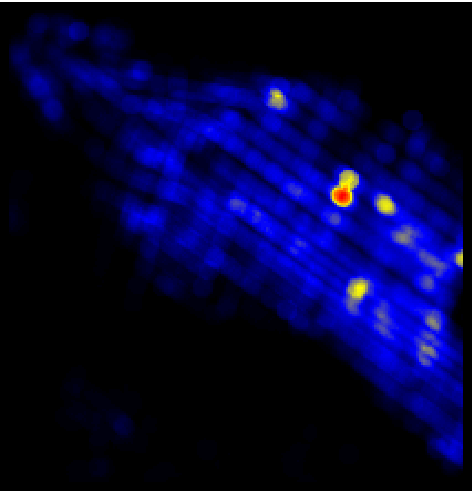
\includegraphics[width=\linewidth]{images/gen-raw-blur-gstar-2}
    \label{fig:BlurExample:a}
  \end{subfigure}
  \begin{subfigure}{.3\linewidth}
    \caption{Large matrix}
    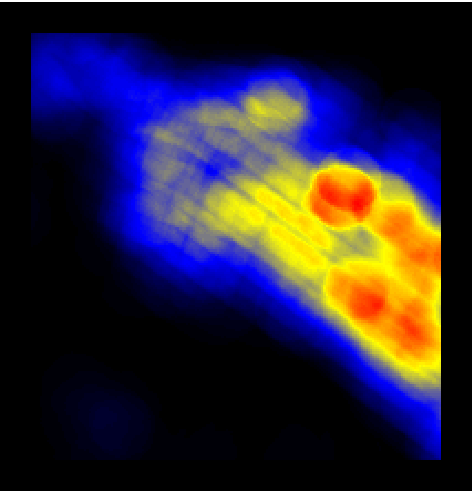
\includegraphics[width=\linewidth]{images/gen-raw-blur-gstar-8}
    \label{fig:BlurExample:b}
  \end{subfigure}
  \caption{
    Example of G* statictics computed for the same raster with different weight 
    matrix sizes.
  }
\end{figure}


We define a hot spot found in comparably more coarse resolutions as
\emph{parent} (larger weight matrix or larger pixel size) and in finer
resolutions as \emph{child} (smaller weight matrix or smaller pixel size).

Stability assumes that every parent has at least one child and that each child
has one parent. For a perfectly stable interaction, it can be easily seen that
the connection between parent and child is a injective function and between
child and parent a surjective function. To measure the stability,
we propose a metric called the \emph{Stability of Hot spot} (SoH). It measures
the deviation from a perfectly stable transformation between the parent and 
chaild rasters (like frames of an animation).

In its downward property (from parent to child, injective) it is defined as:
\begin{equation}
  \label{eq:SoH-down}
  \SOHDOWN
    = \frac{ParentsWithChildNodes}{Parents}
    = \frac{|Parents \cap Children|}{|Parents|}
\end{equation}
And for its upward property (from child to parent, surjective):
\begin{equation}
  \label{eq:SoH-up}
  \SOHUP
    = \frac{ChildrenWithParent}{Children}
    = 1 - \frac{|Children - Parents|}{|Children|}
\end{equation}
where $ParentsWithChildNodes$ is the number of parents that have at least one 
\emph{child}, $Parents$ is the total number of \emph{parent}, 
$ChildrenWithParent$ is the number of children and $Children$ as the total 
number of children.
The SoH is defined for a range between 0 and 1, where 1 represents a perfectly 
stable transformation while 0 would be a transformation with no stability at 
all.
If $|Children|=0$ or $|Parents|=0$ SoH is 0.


%\section{Focal Getis-Ord}
%\label{sec:FocalGetisOrd}
%
%In paper~\cite{SoH-GI-Forum}, we have defined the measure Focal G*.
%We use the notation \FOCAL{R}{M}{op} to denote a focal
%operation $op$ applied on a raster $R$ with a focal window determined by a
%matrix $M$. This is rougly eqivalent to a command \verb|focal(x=R, w=M, 
%fun=op)|
%from package \emph{raster} in the R programming language \cite{cran:raster}.

%\begin{definition}[$G^*$ function on rasters]
%  \label{def:GenericGetisOrdFunc}
%  
%  The function $G^*$ can be expressed as a raster operation:
%  
%  \begin{displaymath}
%    G^*(R, W, st) =
%    \frac{
%      \FOCAL{R}{W}{sum} - M*\sum_{w \in W}{w}
%    }{
%      S \sqrt{
%        \frac{
%          N*\sum_{w \in W}{w^2} - (\sum_{w \in W}{w})^2
%        }{
%          N - 1
%        }
%      }
%    }
%  \end{displaymath}
%  \noindent where:
%  \begin{itemize}
%    
%    \item $R$ is the input raster.
%    
%    \item $W$ is a weight matrix of values between 0 and 1.
%    
%    \item $st = (N, M, S)$ is a parametrization specific to a particular 
%version
%    of the $G^*$ function. (Def.\vref{def:StdGetisOrdVersion} and
%    \vref{def:FocalGetisOrdVersion}).
%    
%  \end{itemize}
%\end{definition}
%
%\begin{definition}[Standard $G^*$ parametrization]
%  \label{def:StdGetisOrdVersion}
%  
%  Computes the parametrization $st$ as global statistics for all pixels in the
%  raster $R$:
%  
%  \begin{itemize}
%    \item $N$ represents the number of all pixels in $R$.
%    \item $M$ represents the global mean of $R$.
%    \item $S$ represents the global standard deviation of all pixels in $R$.
%  \end{itemize}
%\end{definition}
%
%\begin{definition}[Focal $G^*$ parametrization]
%  \label{def:FocalGetisOrdVersion}
%  
%  Let $F$ be a boolean matrix such that: $all(dim(F) \geq dim(W))$.
%  This version uses focal operations to compute per-pixel statistics given by 
%  the focal neighbourhood $F$ as follows:
%  
%  \begin{itemize}
%    
%    \item $N$ is a raster computed as a focal operation \FOCAL{R}{F}{sum}. Each
%    pixel represents the number of pixels from $R$ convoluted with the matrix
%    $F$. 
%    
%    \item $M$ is a raster computed as a focal mean \FOCAL{R}{F}{mean}, thus 
%each
%    pixel represents a mean value of its $F$-neighbourhood.
%    
%    \item $S$ is a raster computed as a focal standard deviation
%    \FOCAL{R}{F}{sd}, thus each pixel represents a standard deviation of its
%    $F$-neighbourhood.
%    
%  \end{itemize}
%  
%\end{definition}



\section{Evaluation}

\subsection{Dataset}

We evaluate our data on the New York city yellow cab data set 
\footnote{$http://www.nyc.gov/html/tlc/html/about/trip\_record\_data.shtml$}. 
This data set includes all taxi drives from the yellow cabs in New York City, 
from location, to passengers and many more informations. In this study, we compare the 
total pickups over January from 2016 in the Manhattan area. 
The borders of the rasters are (40.699607 \textdegree  (N), -74.020265 \textdegree  (E)) 
and (40.769239 \textdegree  (N), -73.948286 \textdegree  (E)) after WGS84.
By using this data set, we reduce the computational effort while still 
being able to show the applicability on real world data and problems.
\subsection{Treatments}

%\begin{definition}[Evaluation Run]
%  \label{def:EvalRun}
%  We define a single evaluation run as a tuple:
%  \begin{displaymath}
%    E = (V, m, p, w)
%  \end{displaymath}
%  \noindent where:
%  \begin{itemize}
%  
%    \item $V$ is the input dataset of points, representing the taxi dropoffs 
%in 
%    our case.
%    
%    \item $m$ is the metric used, in our case either \SOHUP or \SOHDOWN.
%    
%    \item $p$ represents the pixel size for aggregating points from $V$, 
%    e.g. $100 \times 100$ meters.
%    
%    \item $w$ represents the size of a weight matrix.
%    In our case, we chose a weight matrix depicted in 
%    Figure~\ref{fig:ExampleMatrices}(a) for both the G* and FocalG* cases.
%  \end{itemize}
%\end{definition}

%Figure~\ref{fig:ComparisonMorning} and Figure~\ref{fig:ComparisonEvening} show
%Standard and Focal $G^*$ computations for both morning and eventing datasets
%with weight matrix $W$ of size 3, 5, 7, 9, 15 and 31. In this figures, when 
%computing Focal
%$G^*$, the focal matrix $F$ has a constant size of $61{\times}61$ cells. 
%Example weight matrix $W$ and focal matrix $F$ are depicted in 
%Figure~\ref{fig:ExampleMatrices}.

Aggregation size 1 means we aggregate every point, which was in range of $100x100 \cdot 0.000001$ into one pixel. 
For aggregation size Z we aggregated ZxZ pixel from aggregated size 1 into a new pixel.
%
For our measurements we specified the following data series:
\begin{itemize}
 \item $W_i$: The weight matrix W is from 3 to 47 with a stepsize of 4.
 \item $F_j$: The focal matrix F is from  17 to 137 with a stepsize of 12. F is ignored for $G^*$ but not for Focal $G^*$
 \item $R_z$: The aggregation level is from 1 to 6 with a stepsize of 1. R represents the raster
\end{itemize}
\begin{definition}

  \begin{displaymath}
    \SOHUP(child, parent)
  \end{displaymath}
  \begin{displaymath}
    \SOHDOWN(child, parent)
  \end{displaymath}
  
  The SoH for a singled evalution run in the weight dimension is defined as:
  \begin{eqnarray*}
    child & = & G^*(R_z, W_{3+i \cdot 4}, st, F_{17+j \cdot 12}) \\
    parent & = & G^*(R_z, W_{3+(i+1) \cdot 4}, st, F_{17+j \cdot 12}) )
  \end{eqnarray*}
  The SoH for a singled evalution run in the focal dimension is defined as:
  \begin{eqnarray*}
    child & = & G^*(R_z, W_{3+i \cdot 4}, st, F_{17+j \cdot 12}) \\
    parent & = & G^*(R_z, W_{3+i \cdot 4}, st, F_{17+(j+1) \cdot 12}) )
  \end{eqnarray*}
  The SoH for a singled evalution run in the aggregation dimension is defined 
  as:
  \begin{eqnarray*}
    child & = & G^*(R_z, W_{3+i \cdot 4}, st, F_{17+j \cdot 12}) \\
    parent & = & G^*(R_{z+1}, W_{3+i \cdot 4}, st, F_{17+j \cdot 12}) )
  \end{eqnarray*}
  
  
  \begin{displaymath}
  z \in [1,6], i,j \in [0,10], G^* \in [Standard, Focal]
  \end{displaymath}
\end{definition}

Therefore we would calculate $10 \cdot 10 \cdot 5 + 10 \cdot 5=550$ results for each dimension.
The following conditions must hold $dim(F) > dim(W)$ and $dim(F) < dim(R)$ 
which leads e.g. to 460 results in the z-dimension.
We vary over the weight matrix W, the focal matrix F and the aggregation level, as motivated in the introduction.
To compare the impact each of these parameters has we compute all variations 
over two parameter and holding one parameter fix. We then calculate the mean as 
well as the standard deviation for the SoH for the fixed value based on the two 
other parameters. This allows us to isolate the impact of the variation in the 
single parameter. The results are then plotted in 
Figures~\ref{fig:SoHFocal}--\ref{fig:SoHZoom}, one image for each fixed 
parameter and the direction of the SoH.
The hotspots to use the SoH on are computed by the focal $G^*$ and standard $G^*$ method. The focal $G^*$ allows us, to isolate the impact that the size of the study area has on the stability of the results without recomputing the total dataset. 
\subsection{Clumping}

The SoH needs a parent and a child. Clusters can be calculated different. For
$G^*$ a sigmoid can be used. Values above 2.58 and under -2.58 means in less
then 1\% of the cases you are wrong. The values of Focal $G^*$ depend on the
focal size F. Therefore, we decide all values in the top quantile belong to a
clusters. For clustering we grouped the neighbourhood with values in the top
quantile to one cluster. Neigbours are are pixels with touching edges which
leads for every pixel to 8 neigbours. Fig.~\ref{fig:Clumping} depicts the 
clusters using different colours. In this figure, Focal~$G^*$ has smaller 
clusters which are distributed over the complete raster.

\begin{figure}[htp]
  \centering
  
  \begin{subfigure}{.7\linewidth}
    \caption{G* clustering difference}
    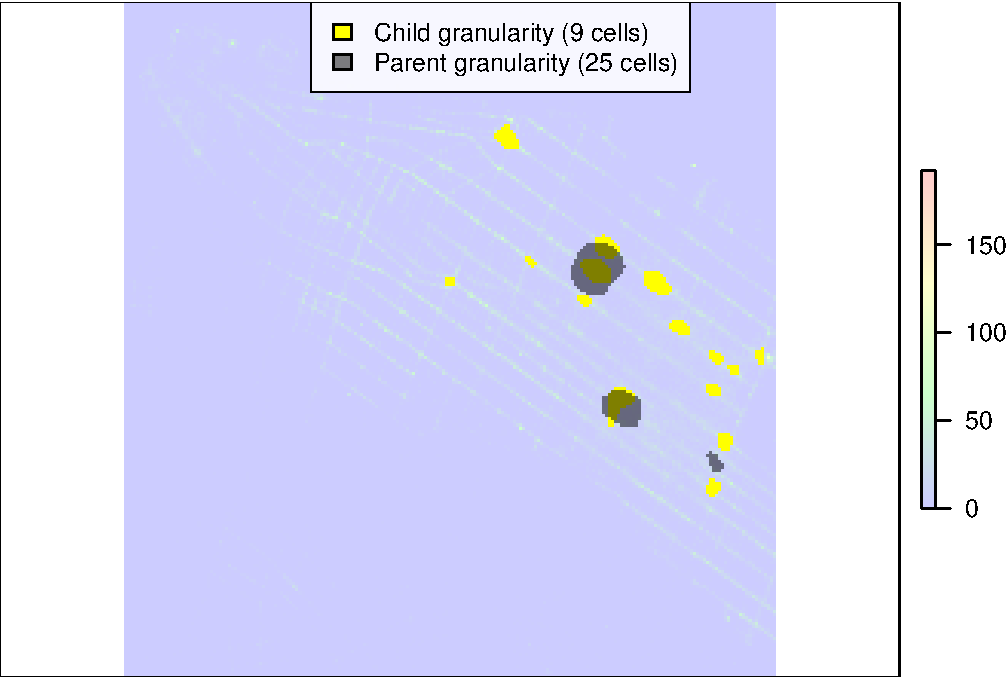
\includegraphics[width=\linewidth]{images/gen-metric-example-1}
    \label{fig:ClustDiffGstar}
  \end{subfigure}
  \hspace{3em}
  \begin{subfigure}{.7\linewidth}
    \caption{Focal G* clustering difference}
    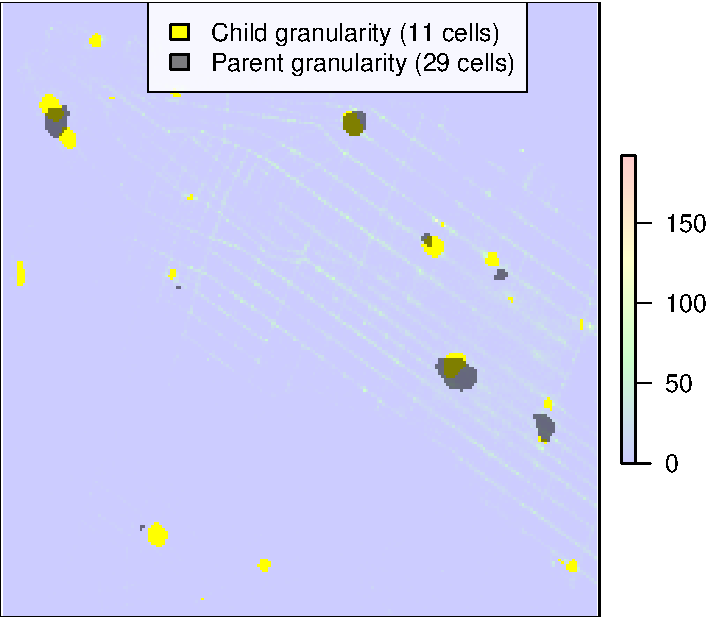
\includegraphics[width=\linewidth]{images/gen-metric-example-2}
    \label{fig:ClustDiffFocalGstar}
  \end{subfigure}
  
  \caption{
    Example clustering for G* and Focal G* used as a input for SoH computation.
  }
  \label{fig:Clumping}
\end{figure}


\subsection{Aggregate}

The aggregation level is a slice plane through our three dimensional space. 
This is an example how the results can look with visualize representations of the calculated 
rasters and the raw data.
\begin{definition} Aggregation run:
\begin{eqnarray*}
    child & = & G^*(R_z, W_{11}, st, F_{41}) \\
    parent & = & G^*(R_{z+1}, W_{11}, st, F_{41})
  \end{eqnarray*}
\begin{displaymath}
z \in [1,6], G^* \in [Standard, Focal]
\end{displaymath}
\end{definition}

The results can be found in Figure~\ref{fig:Zoom}. It can be seen that with an
increase of the aggregation level the values increase. 
%TODO: there was some todo in the text for the following sentence
If clusters
increase/decrease For the upward property, $G^*$ is always better than Focal
$G^*$, compared to the results from figure \ref{fig:SoHZoom}. Focal $G^*$
reaches the same result as $G^*$ at aggregation level~5 . For the downward
property, Focal $G^*$ leads to better results at aggregation level~5.

\begin{figure*}[htp]
  \centering
  \begin{tabular}{cccccccc}
    \multicolumn{8}{l}{
      Aggregation levels computed from original raster (log scale)
    }\\
    \hline
    1 & 2 & 3 & 4 & 5 & 6 & 7 & 8 \\
    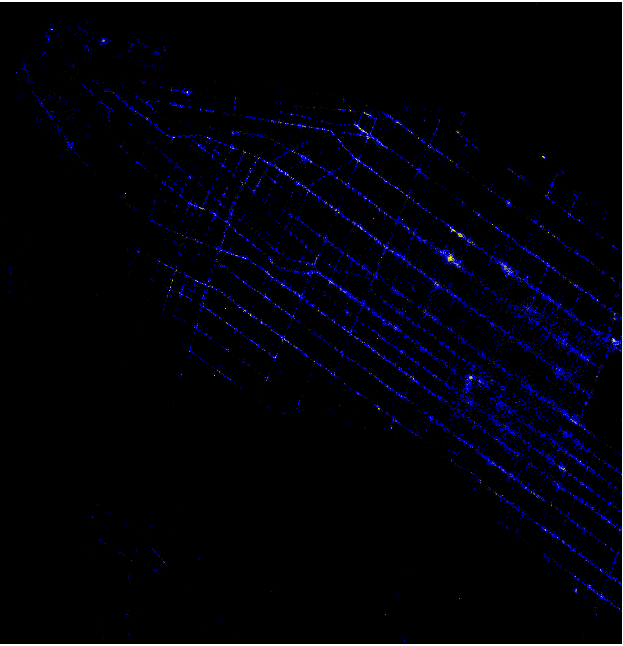
\includegraphics[width=4.6em]{images/gen-rawdata-1}&
    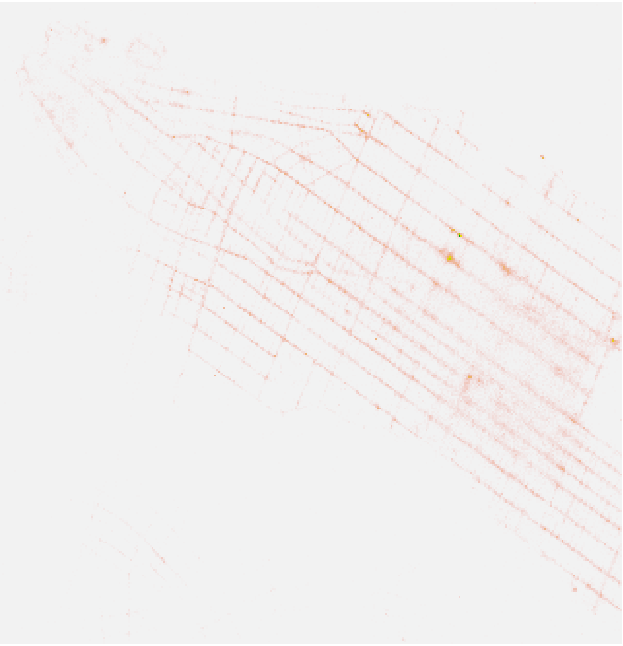
\includegraphics[width=4.6em]{images/gen-rawdata-2}&
    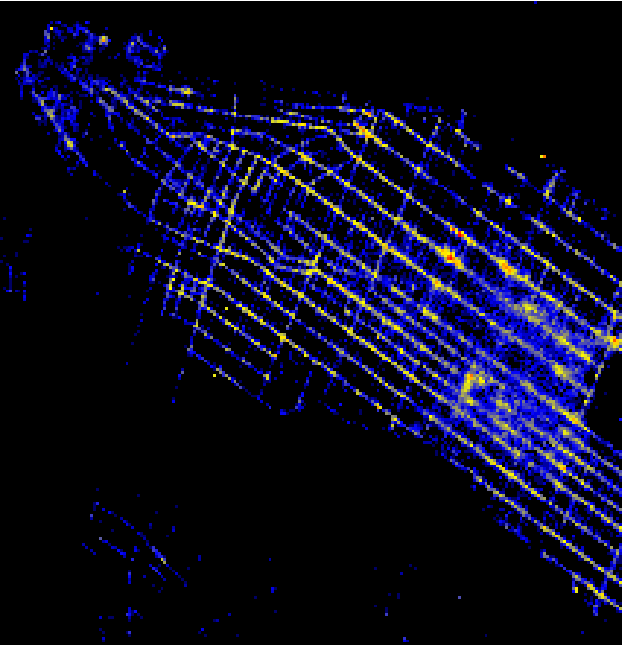
\includegraphics[width=4.6em]{images/gen-rawdata-3}&
    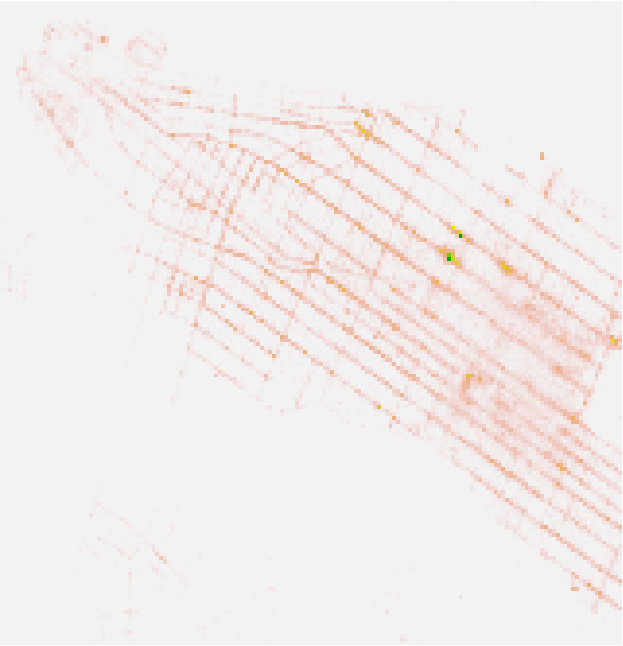
\includegraphics[width=4.6em]{images/gen-rawdata-4}&
    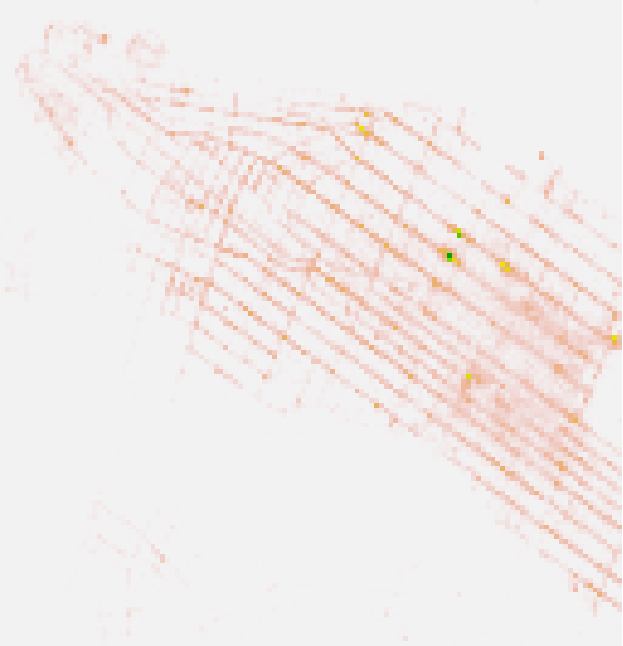
\includegraphics[width=4.6em]{images/gen-rawdata-5}&
    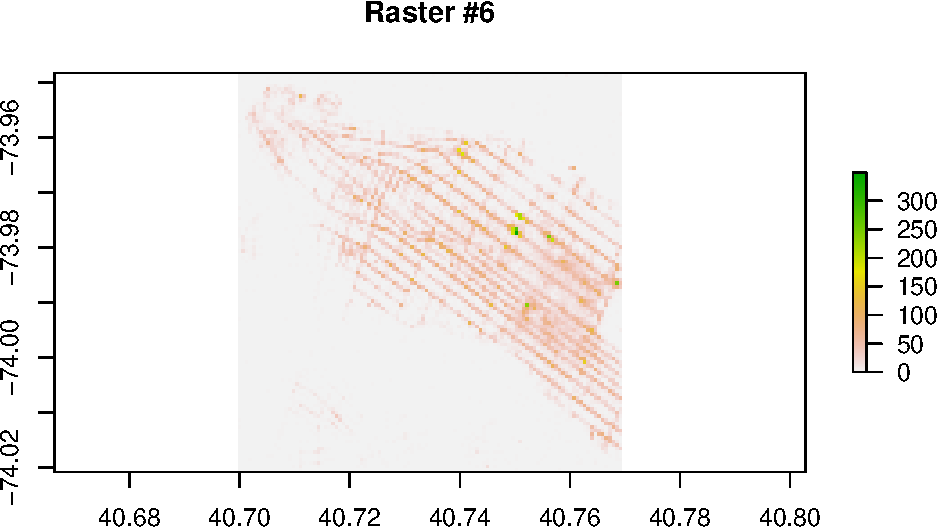
\includegraphics[width=4.6em]{images/gen-rawdata-6}&
    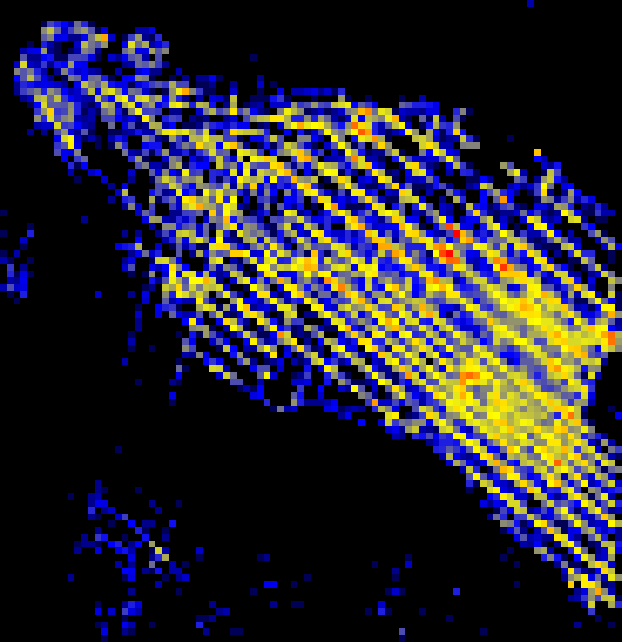
\includegraphics[width=4.6em]{images/gen-rawdata-7}&
    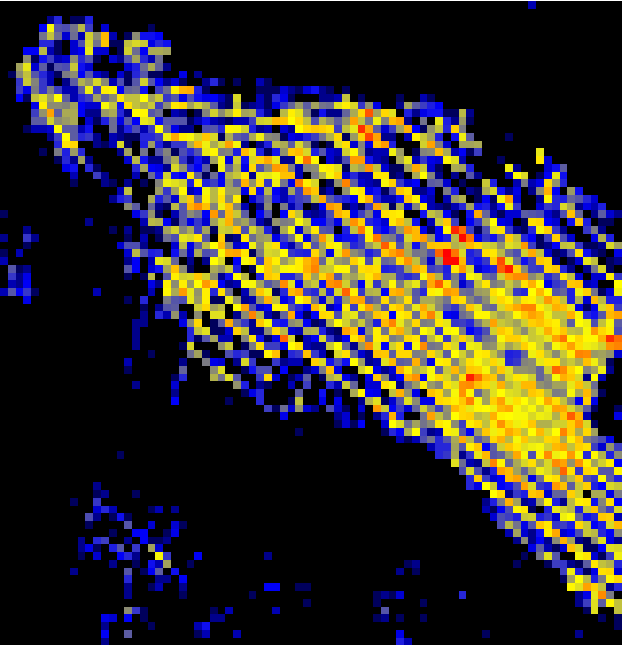
\includegraphics[width=4.6em]{images/gen-rawdata-8}
  \end{tabular}
  
  \vspace{1em}
  \begin{tabular}{cccccccc}
    \multicolumn{8}{l}{G* computed from multiple aggregation levels} \\
    \hline
    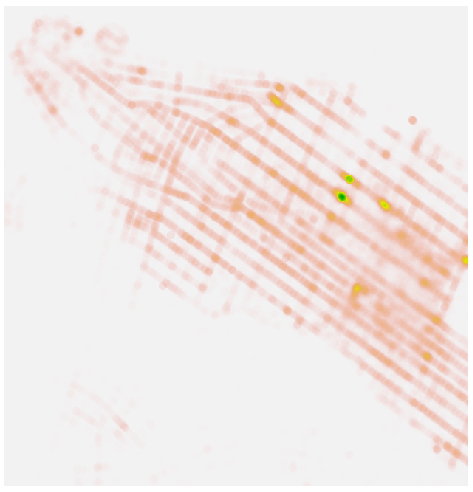
\includegraphics[width=4.6em]{images/gen-raw-zoom-gstar-1}&
    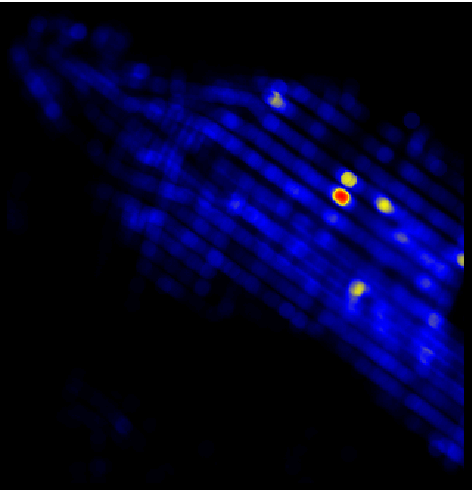
\includegraphics[width=4.6em]{images/gen-raw-zoom-gstar-2}&
    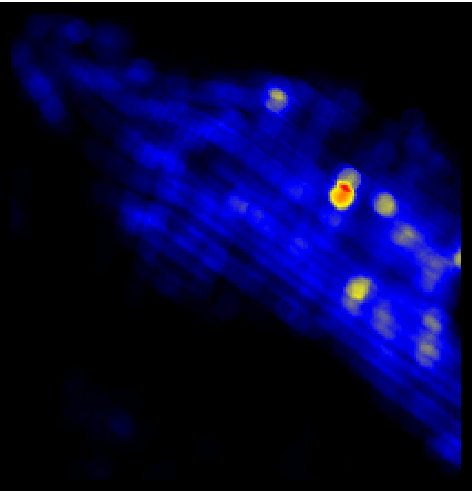
\includegraphics[width=4.6em]{images/gen-raw-zoom-gstar-3}&
    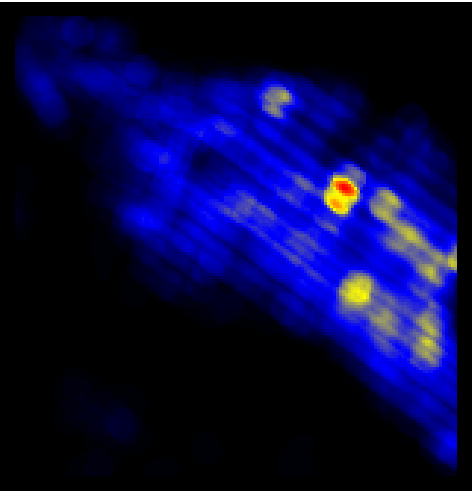
\includegraphics[width=4.6em]{images/gen-raw-zoom-gstar-4}&
    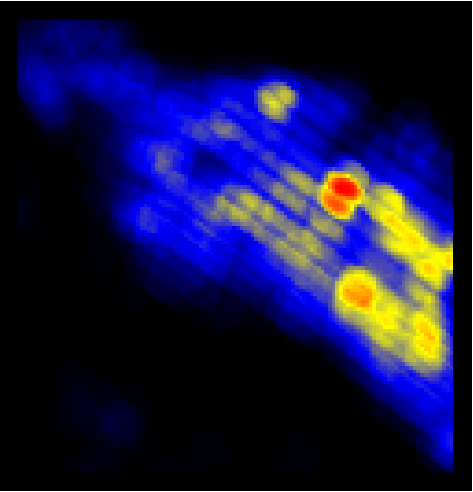
\includegraphics[width=4.6em]{images/gen-raw-zoom-gstar-5}&
    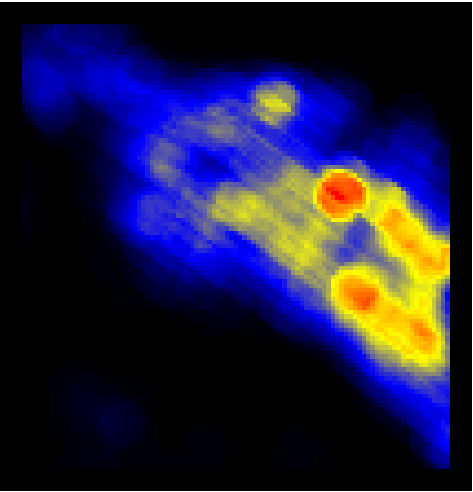
\includegraphics[width=4.6em]{images/gen-raw-zoom-gstar-6}&
    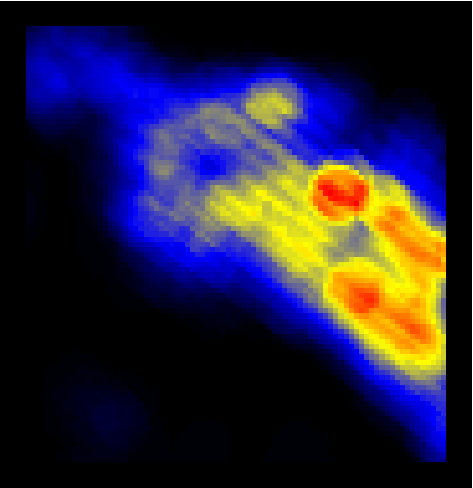
\includegraphics[width=4.6em]{images/gen-raw-zoom-gstar-7}&
    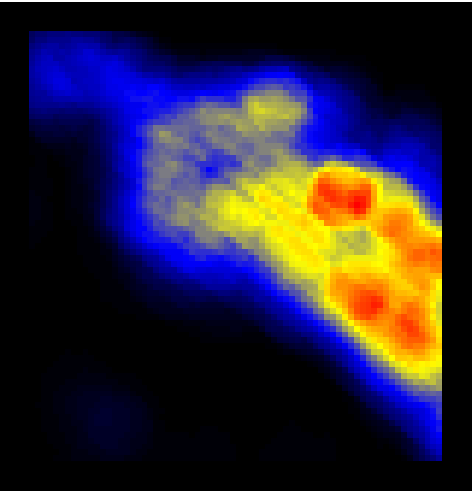
\includegraphics[width=4.6em]{images/gen-raw-zoom-gstar-8}\\
    
    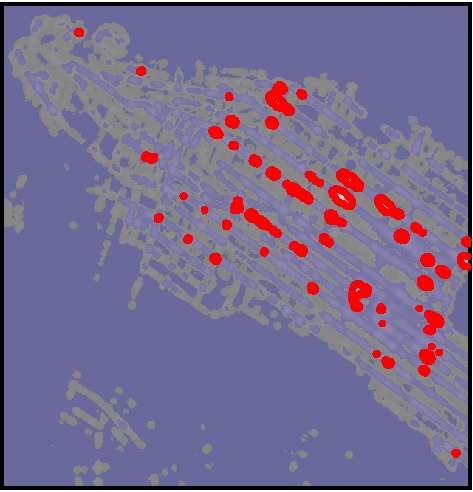
\includegraphics[width=4.6em]{images/gen-demo-zoom-gstar-1}&
    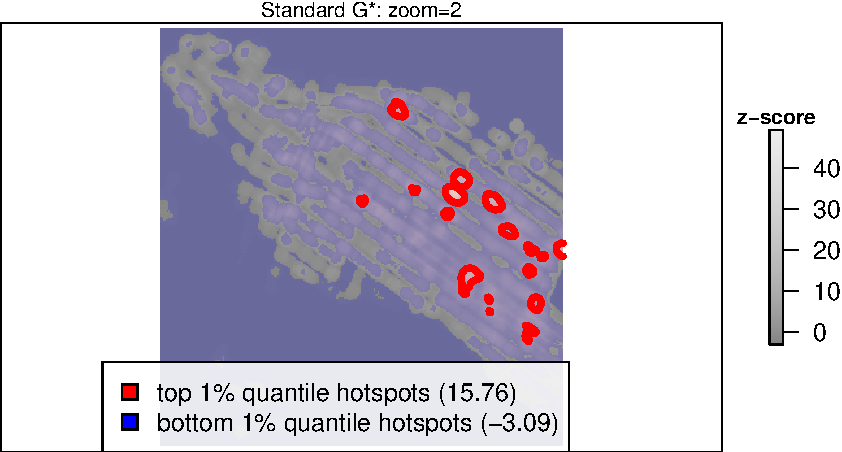
\includegraphics[width=4.6em]{images/gen-demo-zoom-gstar-2}&
    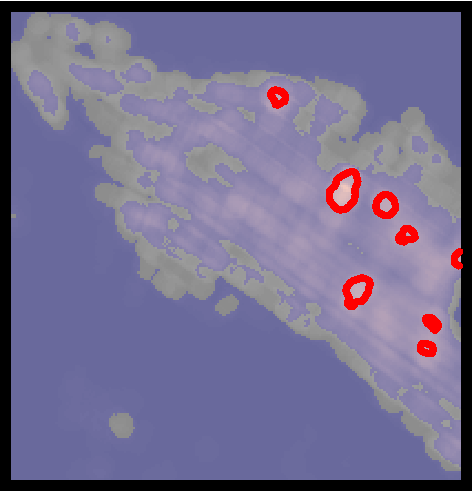
\includegraphics[width=4.6em]{images/gen-demo-zoom-gstar-3}&
    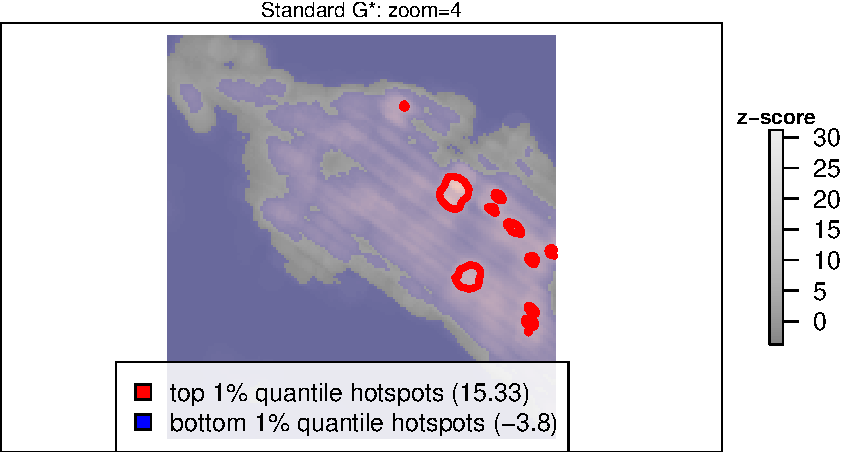
\includegraphics[width=4.6em]{images/gen-demo-zoom-gstar-4}&
    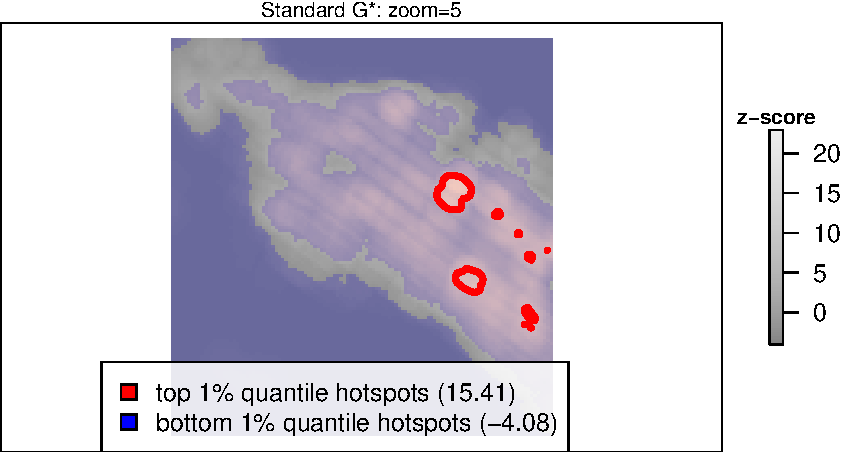
\includegraphics[width=4.6em]{images/gen-demo-zoom-gstar-5}&
    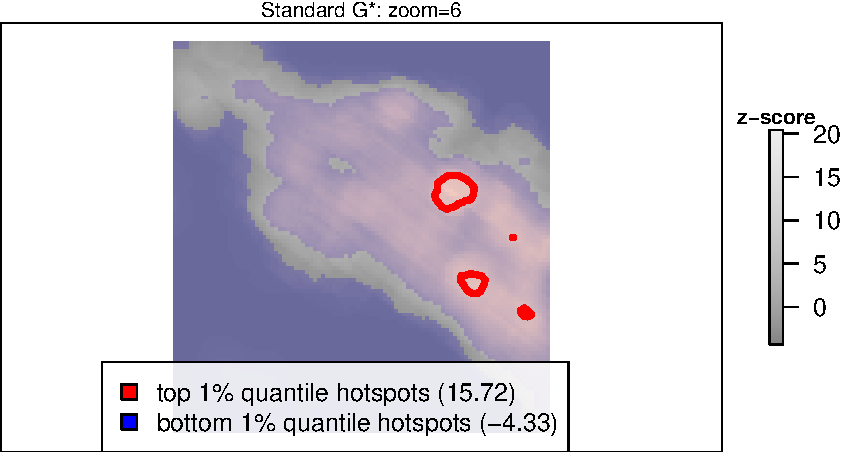
\includegraphics[width=4.6em]{images/gen-demo-zoom-gstar-6}&
    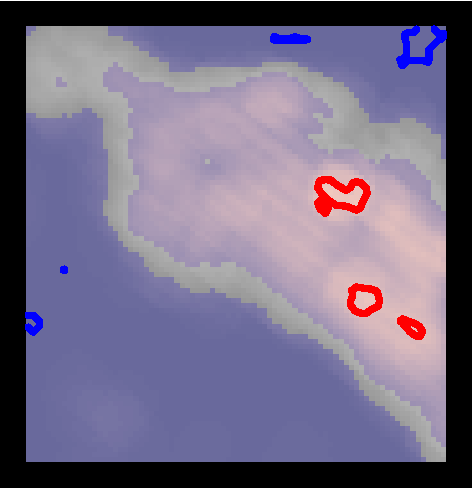
\includegraphics[width=4.6em]{images/gen-demo-zoom-gstar-7}&
    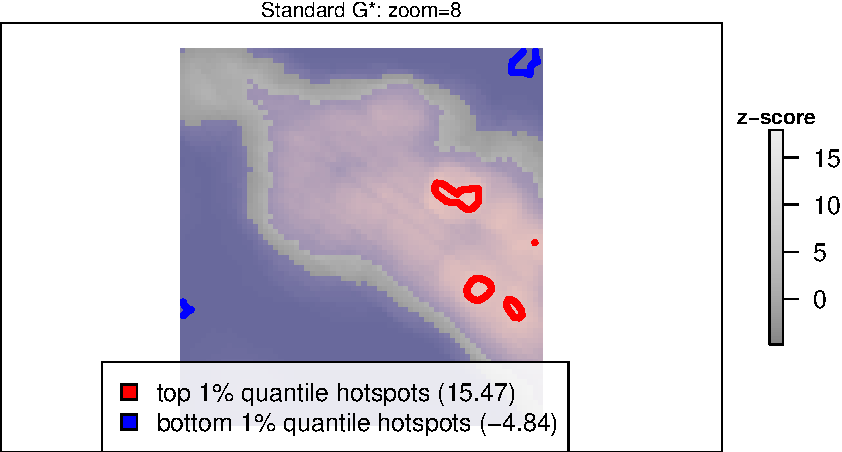
\includegraphics[width=4.6em]{images/gen-demo-zoom-gstar-8}\\
    
  \end{tabular}
  
  \vspace{1em}
  \begin{tabular}{cccccccc}
    \multicolumn{8}{l}{Focal G* computed from multiple aggregation levels} \\
    \hline
    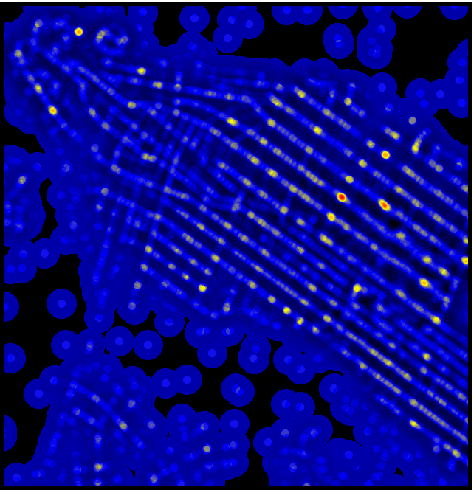
\includegraphics[width=4.6em]{images/gen-raw-zoom-focalgstar-1}&
    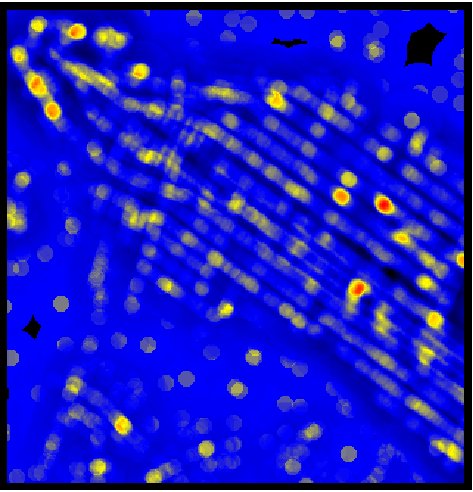
\includegraphics[width=4.6em]{images/gen-raw-zoom-focalgstar-2}&
    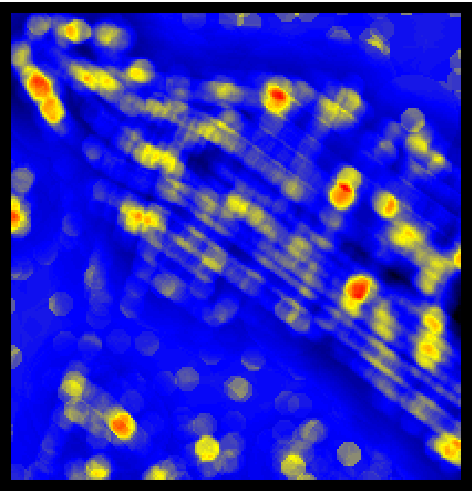
\includegraphics[width=4.6em]{images/gen-raw-zoom-focalgstar-3}&
    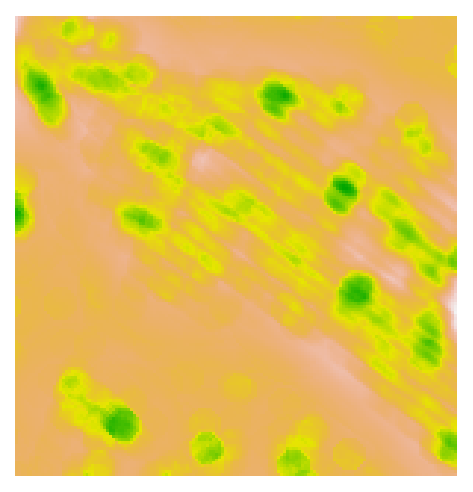
\includegraphics[width=4.6em]{images/gen-raw-zoom-focalgstar-4}&
    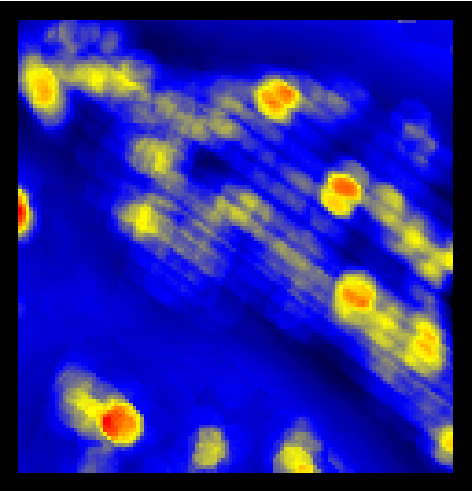
\includegraphics[width=4.6em]{images/gen-raw-zoom-focalgstar-5}&
    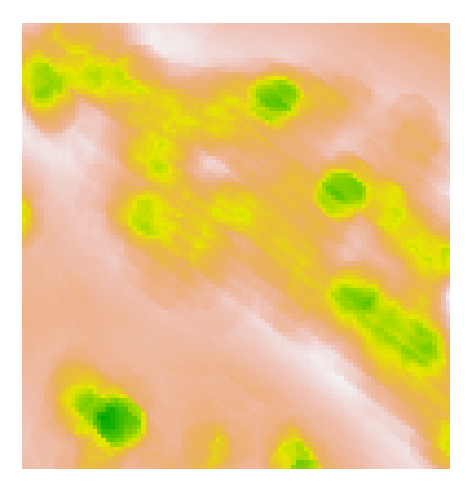
\includegraphics[width=4.6em]{images/gen-raw-zoom-focalgstar-6}&
    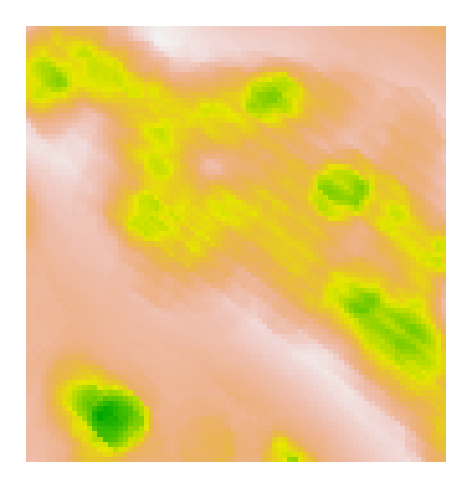
\includegraphics[width=4.6em]{images/gen-raw-zoom-focalgstar-7}&
    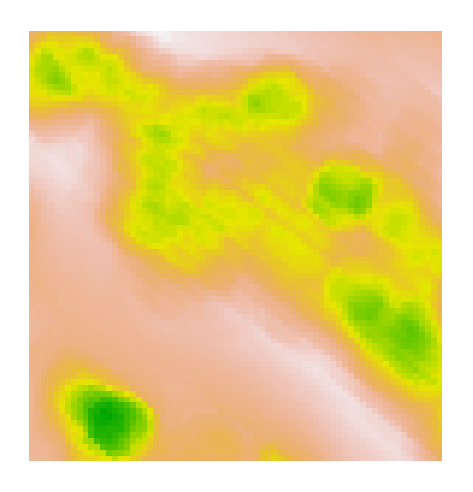
\includegraphics[width=4.6em]{images/gen-raw-zoom-focalgstar-8}\\
    
    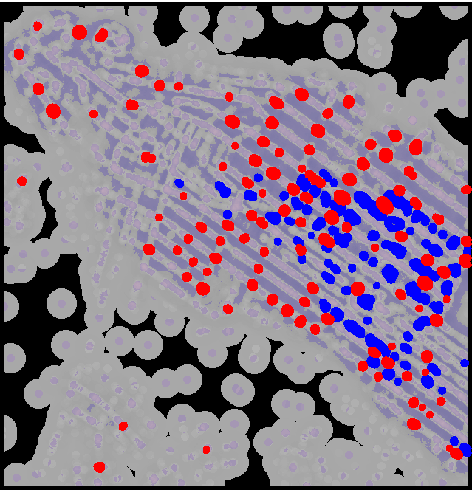
\includegraphics[width=4.6em]{images/gen-demo-zoom-focalgstar-1}&
    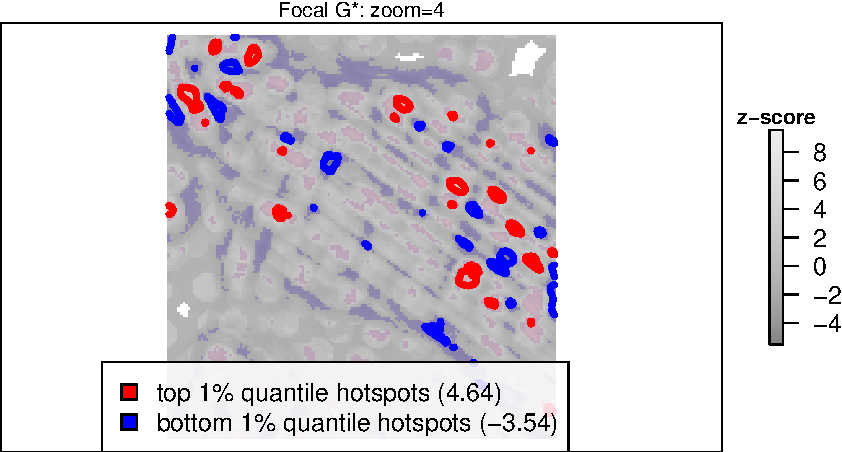
\includegraphics[width=4.6em]{images/gen-demo-zoom-focalgstar-2}&
    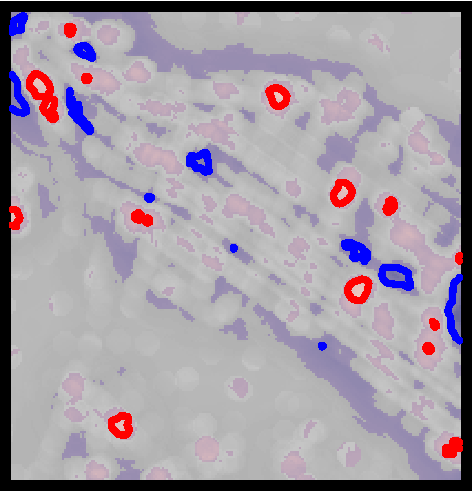
\includegraphics[width=4.6em]{images/gen-demo-zoom-focalgstar-3}&
    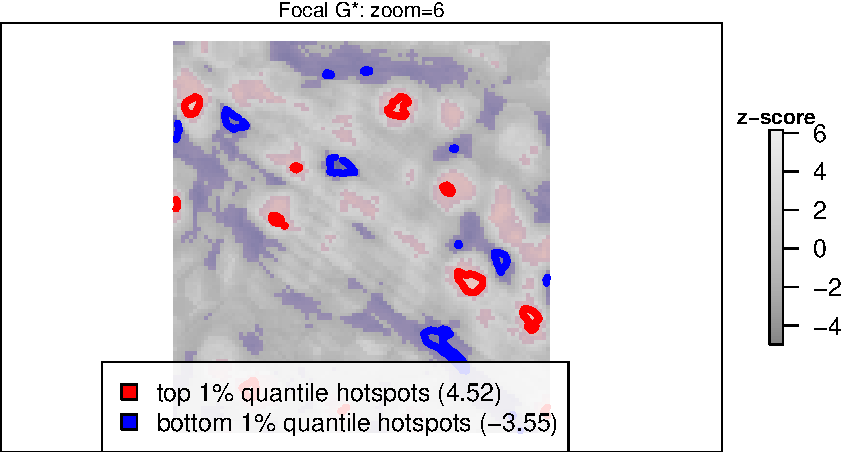
\includegraphics[width=4.6em]{images/gen-demo-zoom-focalgstar-4}&
    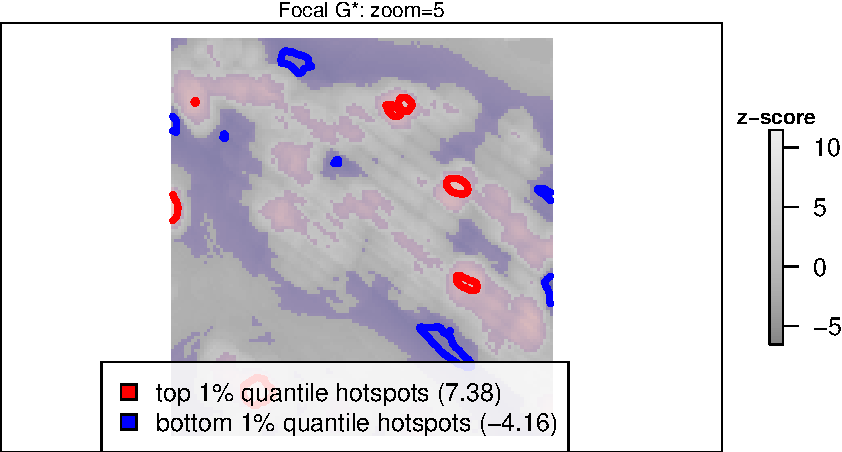
\includegraphics[width=4.6em]{images/gen-demo-zoom-focalgstar-5}&
    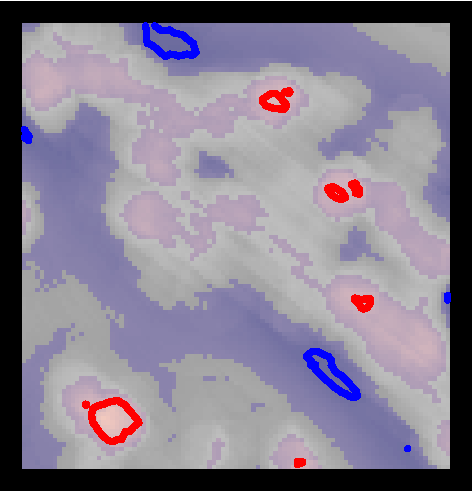
\includegraphics[width=4.6em]{images/gen-demo-zoom-focalgstar-6}&
    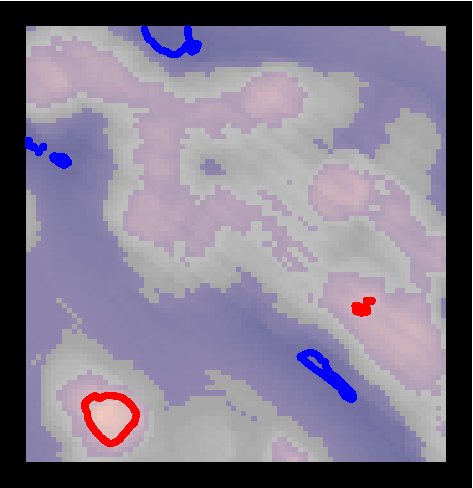
\includegraphics[width=4.6em]{images/gen-demo-zoom-focalgstar-7}&
    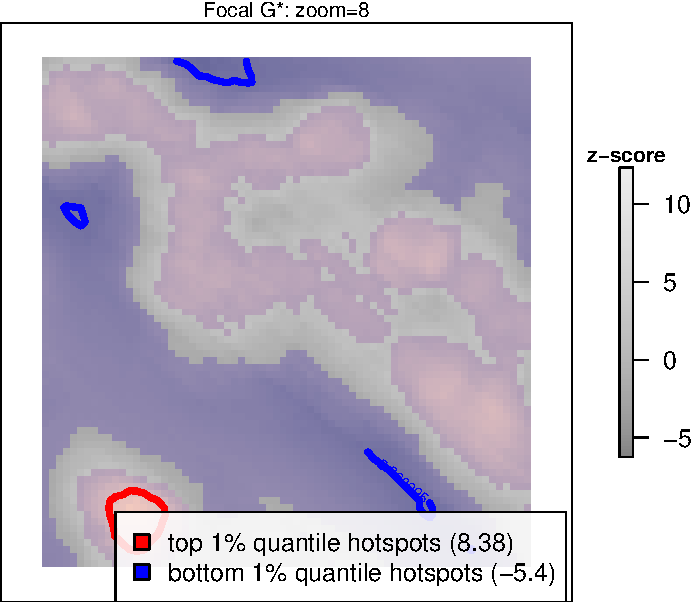
\includegraphics[width=4.6em]{images/gen-demo-zoom-focalgstar-8}\\
  \end{tabular}
  
  \vspace{2em}
  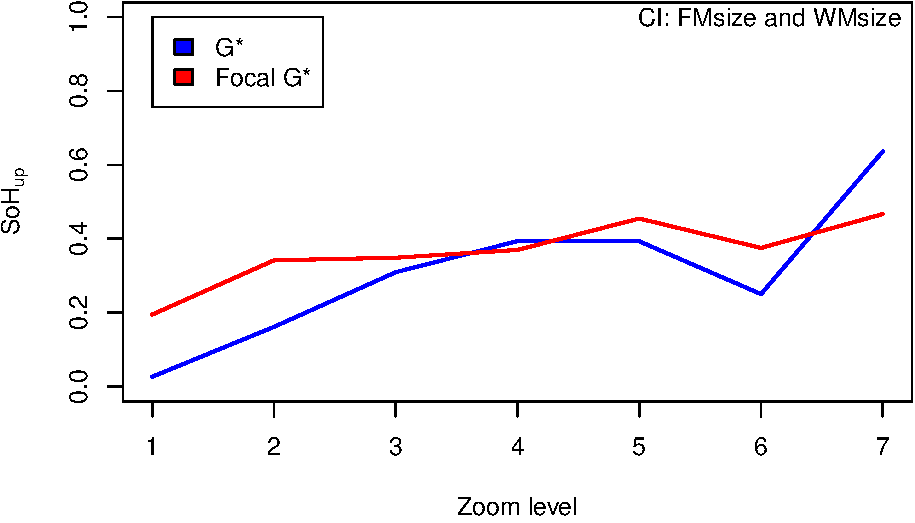
\includegraphics[width=.45\linewidth]{images/gen-zoom-sohup-1}
  \hspace{1em}
  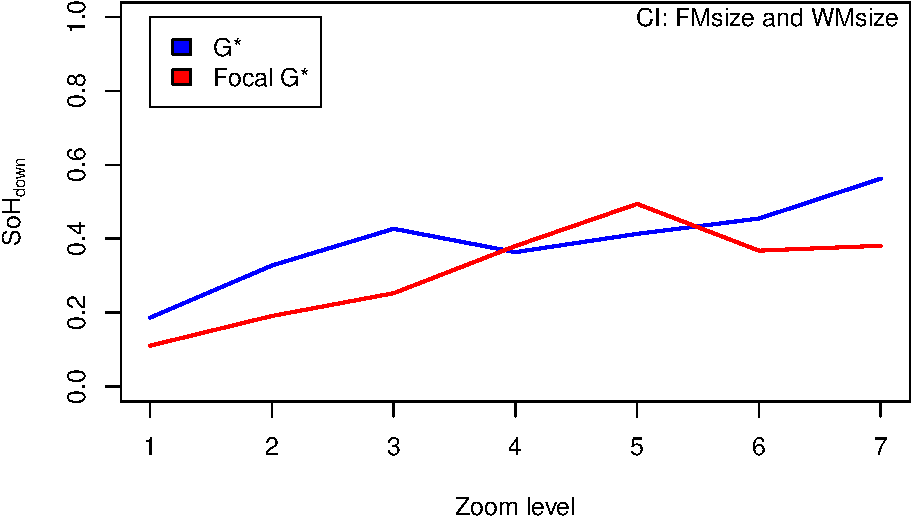
\includegraphics[width=.45\linewidth]{images/gen-zoom-sohdown-1}
  
  \caption{
    This image shows all aggregation levels for G* and Focal G* together 
    with two metrics -- $SoH^\uparrow$ and $SoH^\downarrow$.
  }
  \label{fig:Zoom}
\end{figure*}

\subsection{Blur}
We also made an example for the variation of the weight size W.
Blur is a slice plane through our three dimensional space. 
W is changed from 7 to 29 with a stepsize of 2, F and the aggregation level is fixed.
\begin{definition} Blur run:
\begin{eqnarray*}
    child & = & G^*(R_3, W_{7+i \cdot 2}, st, F_{41}) \\
    parent & = & G^*(R_3, W_{7+(i+1)\cdot 2}, st, F_{41})
  \end{eqnarray*}
\begin{displaymath}
i \in [0,11], G^* \in [Standard, Focal]
\end{displaymath}
\end{definition}
The blur results are plotted in Figure~\ref{fig:Blur}. The weight matrix is
shown in the first row, with increasing size. The 2nd and 3th row show how
$G^*$ and Focal $G^*$ changes based on W. This example is a slice plane of the
weight dimension ploted in figure ~\ref{fig:SoHWeight}. It can be seen that an
increase of the weight size leads in general to better results for Focal $G^*$.


\begin{figure*}[htp]
  \centering
  \begin{tabular}{cccccccc}
    \multicolumn{8}{l}{Multiple weight matrix sizes} \\
    \hline
    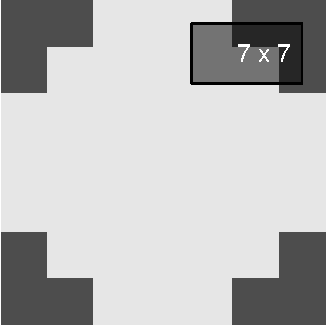
\includegraphics[width=4.6em]{images/gen-blur-wmatrices-1}&
    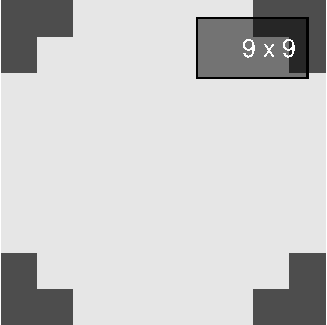
\includegraphics[width=4.6em]{images/gen-blur-wmatrices-2}&
    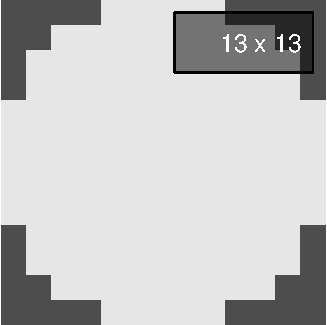
\includegraphics[width=4.6em]{images/gen-blur-wmatrices-3}&
    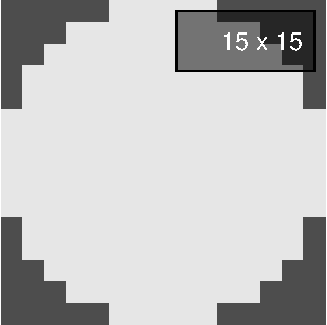
\includegraphics[width=4.6em]{images/gen-blur-wmatrices-4}&
    \includegraphics[width=4.6em]{images/gen-blur-wmatrices-5}&
    \includegraphics[width=4.6em]{images/gen-blur-wmatrices-6}&
    \includegraphics[width=4.6em]{images/gen-blur-wmatrices-7}&
    \includegraphics[width=4.6em]{images/gen-blur-wmatrices-8}
  \end{tabular}
  
  \vspace{1em}
  \begin{tabular}{cccccccc}
    \multicolumn{8}{l}{G* computed using different weight matrix sizes} \\
    \hline
    \includegraphics[width=4.6em]{images/gen-raw-blur-gstar-1}&
    \includegraphics[width=4.6em]{images/gen-raw-blur-gstar-2}&
    \includegraphics[width=4.6em]{images/gen-raw-blur-gstar-3}&
    \includegraphics[width=4.6em]{images/gen-raw-blur-gstar-4}&
    \includegraphics[width=4.6em]{images/gen-raw-blur-gstar-5}&
    \includegraphics[width=4.6em]{images/gen-raw-blur-gstar-6}&
    \includegraphics[width=4.6em]{images/gen-raw-blur-gstar-7}&
    \includegraphics[width=4.6em]{images/gen-raw-blur-gstar-8}\\
    
    \includegraphics[width=4.6em]{images/gen-demo-blur-gstar-1}&
    \includegraphics[width=4.6em]{images/gen-demo-blur-gstar-2}&
    \includegraphics[width=4.6em]{images/gen-demo-blur-gstar-3}&
    \includegraphics[width=4.6em]{images/gen-demo-blur-gstar-4}&
    \includegraphics[width=4.6em]{images/gen-demo-blur-gstar-5}&
    \includegraphics[width=4.6em]{images/gen-demo-blur-gstar-6}&
    \includegraphics[width=4.6em]{images/gen-demo-blur-gstar-7}&
    \includegraphics[width=4.6em]{images/gen-demo-blur-gstar-8}\\
  \end{tabular}

  \vspace{1em}
  \begin{tabular}{cccccccc}
    \multicolumn{8}{l}{Focal G* computed using different weight matrix sizes} \\
    \hline
    \includegraphics[width=4.6em]{images/gen-raw-blur-focalgstar-1}&
    \includegraphics[width=4.6em]{images/gen-raw-blur-focalgstar-2}&
    \includegraphics[width=4.6em]{images/gen-raw-blur-focalgstar-3}&
    \includegraphics[width=4.6em]{images/gen-raw-blur-focalgstar-4}&
    \includegraphics[width=4.6em]{images/gen-raw-blur-focalgstar-5}&
    \includegraphics[width=4.6em]{images/gen-raw-blur-focalgstar-6}&
    \includegraphics[width=4.6em]{images/gen-raw-blur-focalgstar-7}&
    \includegraphics[width=4.6em]{images/gen-raw-blur-focalgstar-8}\\
    
    \includegraphics[width=4.6em]{images/gen-demo-blur-focalgstar-1}&
    \includegraphics[width=4.6em]{images/gen-demo-blur-focalgstar-2}&
    \includegraphics[width=4.6em]{images/gen-demo-blur-focalgstar-3}&
    \includegraphics[width=4.6em]{images/gen-demo-blur-focalgstar-4}&
    \includegraphics[width=4.6em]{images/gen-demo-blur-focalgstar-5}&
    \includegraphics[width=4.6em]{images/gen-demo-blur-focalgstar-6}&
    \includegraphics[width=4.6em]{images/gen-demo-blur-focalgstar-7}&
    \includegraphics[width=4.6em]{images/gen-demo-blur-focalgstar-8}\\
  \end{tabular}
  
  \vspace{2em}
  \includegraphics[width=.45\linewidth]{images/gen-blur-sohup-1}
  \hspace{1em}
  \includegraphics[width=.45\linewidth]{images/gen-blur-sohdown-1}
  
  \caption{
    This image shows different weight matrix sizes for G* and Focal G* together 
    with two metrics -- $SoH^\uparrow$ and $SoH^\downarrow$.
  }
  \label{fig:Blur}
\end{figure*}

\section{Results and Discussion}

% Focal size  
%	Increase of focal size leads to better results in the upward property
% 	Standard deviation decrease with higher focal size 
%	No standard deviation af F 17x17 because of missing clusters
%	The downward property reaches its maximum at 65x65
%
%	Conclusion: F should be around 65x65 or higher
\subsection{Impact of study area}
The first parameter we want to isolate is the size of the study area. This enables us to discuss the optimal size of the study area for the given research/decision question. 
To do so, we have to fix the focal size F and use it as the x-axis and plot the 
mean value as well as the mean +/- the standard deviations of the SoH for all 
other parameter combinations as the y-axis.
In this scenario, only the Focal $G^*$ can produce varied results as the standard $G^*$ has by definition a fixed study area by always using the total size of the study area. 
In Figure~\ref{fig:SoHFocal} the \SOHUP and \SOHDOWN is shown for $G^*$ and 
Focal $G^*$.
Higher values indicate that the hot spots found are more stable. 
The \SOHUP in Figure~\ref{fig:fUp} growth with an increase of the focal size.
It can see that an increase of the focal size leads to better results for \SOHUP. 
With a higher focal size you can see that the dotted line, which represent the standard deviation, is getting smaller. This indicates that an increase in the size of the study area does not only lead to an overall increase of stability but also that the it reduces the volatility of the variations in other parameters.
When F and W have similar size, there are no clusters. Because the values have no much variation. 
\SOHDOWN (Figure ~\ref{fig:fDown}) shows a different picture then the \SOHUP.
It reaches its maximum SoH for a focal size F of 65x65 in our evaluation set. 
The standard deviation is not decreasing with an increase of the 
focal size. 

\begin{figure}[htp]
  \begin{subfigure}{\linewidth}
    \caption{SoH up for focal size}
    \includegraphics[width=\linewidth]{images/gen-focal-1}
    \label{fig:fUp}
  \end{subfigure}
  \hspace{1em}
  \begin{subfigure}{\linewidth}
    \caption{SoH down for focal size}
    \includegraphics[width=\linewidth]{images/gen-focal-2}
    \label{fig:fDown}
  \end{subfigure}
  \caption{SoH for focal matrix size}
  \label{fig:SoHFocal}
\end{figure}

%
% Weight size
%	Increase of weight leads to increase of downward property
%	Small break downs for G* for upward and downward property
%	For the upward property Focal G* is better than G*
%
%	Conclusion: Higher weight size leads to better results. There are parametrisations of Focal G* which are better than G*
\subsection{Impact of Neighbourhood size}
Next, we want to isolate the effect of the neighbourhood size by fixing the weight matrix size W 
and using it as x-axis. With the impact of the weight matrix W we gain information on how far the 
interconnectness is between different points as indicated in \cite{Getis.1992}. 
The results for the weight matrix can be seen in figure ~\ref{fig:wUp} for \SOHUP and figure ~\ref{fig:wDown} for \SOHDOWN.
Here it can be seen that in general for both evaluations metrics as well as the different hot spot methods 
an increase in the size of the weight matrix W leads to more stable results as well as that the Focal $G^*$ 
matrix is slightly more stable in most cases for the mean values. 
An interesting phenomena is the dip in stability for the standard $G^*$ for the value of 39. Despite our 
effort we could not determine the reason behind this result, as no overall trend could be extracted.
The standard deviation shows similar no particular trend, but for the values above 37 is increasing. 
We assume that the reason behind this effect is the inclusion of the water near Manhattan, which leads to a stronger differentiation between areas near water and areas more in the inner city. by increasing the weight matrix, the number of points which are influenced increase in number. The other parameter can regulate this impact and therefore the variance is stronger.  

\begin{figure}[htp]
  \begin{subfigure}{\linewidth}
    \caption{SoH up for weight size}
    \includegraphics[width=\linewidth]{images/gen-weight-1}
    \label{fig:wUp}
  \end{subfigure}
  \hspace{1em}
  \begin{subfigure}{\linewidth}
    \caption{SoH down for weight size}
    \includegraphics[width=\linewidth]{images/gen-weight-2}
    \label{fig:wDown}
  \end{subfigure}
  \caption{SoH for weight size}
  \label{fig:SoHWeight}
\end{figure}
%
% Zoom
%	G* alwas better than Focal G* for upward and downward property
%	Focal G* has different focal sizes because zoom is compared
%	At zoom level 4 G* increase much more than Focal G*
%
%	Conclusion: G* is better than Focal G* in the zoom dimension, but the focal size is fixed. The zoom dimension has the least 
%	influence on the value
\subsection{Impact of Aggregation level}
Finally, we isolate the impact of the different aggregation levels on the stability of the hot spot analysis. 
We fix the aggregation and use it as x-axis. This allows us to examine the impact
the resolution of a data set has on the results and allow us indirectly to reduce the 
computational effort on future computations by using the maximal aggregation as useful.
The results can seen in Figure~\ref{fig:SoHZoom}.
First, we can see that for the aggregation level, in contrast to previous 
results, the standard $G^*$ seems to be more stable.


For the \SOHUP there is a huge increase between aggregation level 4 and 5. This increase can't be seen for \SOHDOWN.
One can see that $G^*$ is always better than Focal $G^*$. 
This could be beacause the target area of Focal $G^*$ increases with every aggregation step. 


\begin{figure}[htp]
  \begin{subfigure}{\linewidth}
    \caption{SoH up for focal size}
    \includegraphics[width=\linewidth]{images/gen-aggregation-1}
    \label{fig:zUp}
  \end{subfigure}
  \hspace{1em}
  \begin{subfigure}{\linewidth}
    \caption{SoH down for focal size}
    \includegraphics[width=\linewidth]{images/gen-aggregation-2}
    \label{fig:zDown}
  \end{subfigure}
  \caption{SoH for focal size}
  \label{fig:SoHZoom}
\end{figure}






\section{Conclusions and Future Work} \label{sec:Conclusion}
In this work we examined the influence of different parameter on the stability
of hot spot analysis on the basis of the Getis-Ord and Focal Getis-Ord
statistic. We validated our results with the use of the SoH metric on a well
known real world data set to ensure external validity and easy replication.
Based on the result we can show several insights, given the restrictions of this
work, for future use of hot spot analysis. First, the greater the area size, the
more stable the results seem to be. The same relation seem to be given for the
size of the weight matrix. The greater the comparable area, the more stable are
the results. Given the study are, the focal range should be at least be a size
of 65x65 tiles, to have a good trade-off between \SOHUP and \SOHDOWN. In the
case of the aggregation level, the stability does not seem to be impacted in the
case of the Focal $G^*$, but for the standard $G^*$ statistic we see an increase
in stability for higher aggregation levels. We assume that the high aggregation
of data and the inherent increase of examined area reduce the impact of
outliers, but reduce the potential to differentiate. The worse results for the
Focal $G^*$ statistic compared to the $G^*$ statistic are most likely a result
of the increased focus on a smaller region. A more in depth look at the
interaction between focal size and aggregation level would be an interesting
question for the future, but this is beyond the scope of this work.

With this work, we made a step further to the optimal parametrisation for $G^*$ 
and Focal $G^*$.
Our results indicate that the parametrization for $G^*$ and Focal $G^*$ besides 
what is defined as parent and child has a huge impact on the
stability of hotspots. We can see the increase of up to 0.6 \SOHUP for e.g. the focal matrix size.
This emphasizes the importance of a metric for the stability of hotspots. But this work also shows the shortcomings of the existing metric, as the trade-off between \SOHUP and \SOHDOWN is not yet fully explored and should be the focus of future work. 
Another interesting field for future research is the stability of spatio-temporal hot spots and their different parametrizations. As $G^*$ is often applied with regard to temporal impacts, the efficient computation of the focal $G^*$ for spatio-temporal and the impact on stability is the second main path for future research. 
We evaluated our data on the aggregate of a single month, but one could assume 
that during the lunchtime there will be hotspots at restaurants and they are 
not 
consistent with the hotspots over one month. Therefore the impact of time on 
the results is important and could also influence the metric for stability in 
profound ways. As in the example, the question is, how fine grained should the 
temporal clustering be and when is the result unstable? 
This leads to the final future work: To which hot spots should the comparison 
be made for the metric? In the current state, only the next parametrization is 
compared due to the high computational complexity. How the comparison of hot 
spots should be carried out and how many different comparisons have to be used 
is another quite interesting research question.

\section{Acknowledgements}
This work is part of the research project BigGIS (reference number: 01IS14012)
funded by the Federal Ministry of Education and Research (BMBF) within the
frame of the programme "Management and Analysis of Big Data" in "ICT 2020 --
Research for Innovations".
%
\noindent R-packages used: \verb|raster|~\cite{cran:raster}, 
\verb|knitr|~\cite{cran:knitr}, 








\bibliographystyle{plain}
\bibliography{bibfile}  % sigproc.bib is the name of the

\end{document}
